\documentclass[tikz]{standalone}
\usepackage{tikz}
\usepackage{pgfplots,graphicx}
\pgfplotsset{compat=newest,compat/show suggested version=false}
\usetikzlibrary{pgfplots.groupplots,matrix}
\usetikzlibrary{positioning,fit,calc,shapes,patterns,automata}
\usepackage{tabularx,xfrac,color,makecell}
\usetikzlibrary{plotmarks}
\usepackage{aurical}
\usepackage[T1]{fontenc}
\usepackage{fontspec}
\newcommand{\lmr}{\fontfamily{lmr}\selectfont} % Latin Modern Roman

\begin{document}
\begin{tikzpicture}
\matrix (m) 
	[
		matrix of nodes,
		nodes=
			{
				draw,
				rectangle,
				ultra thick,
				outer sep=0,
				anchor=center,
				minimum height=4cm,minimum width=4cm
			}
	]
	{
		{
\includegraphics[width=4cm]{mountain.pdf}} & {
\includegraphics[width=4cm]{person.pdf}} & {
\includegraphics[width=4cm]{one.pdf}} & {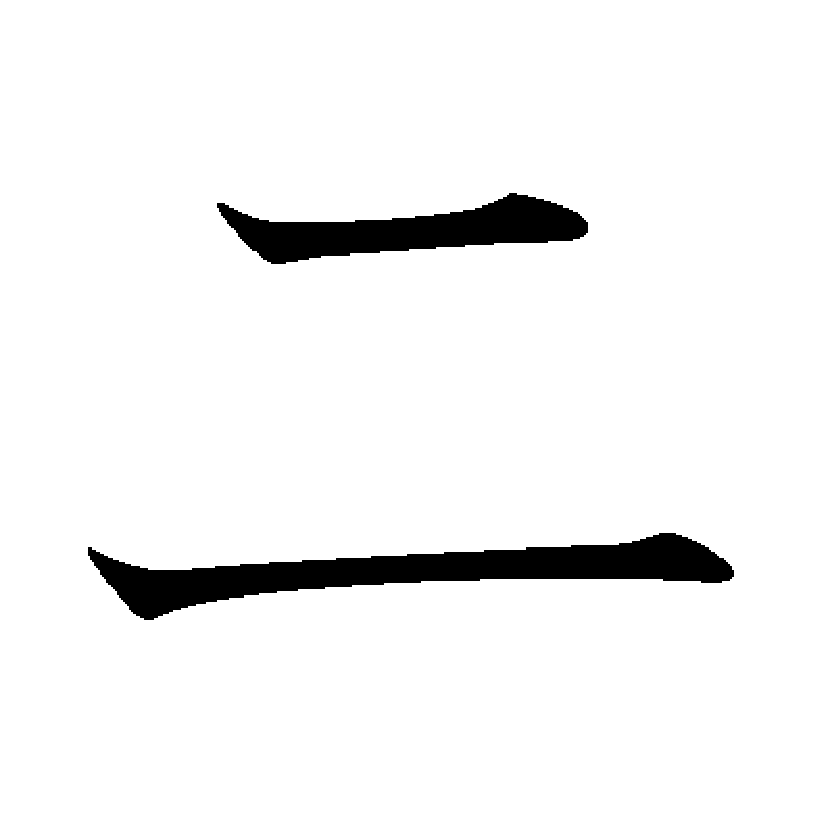
\includegraphics[width=4cm]{two.pdf}} \\
		{
\includegraphics[width=4cm]{three.pdf}} & {
\includegraphics[width=4cm]{sun.pdf}} & {
\includegraphics[width=4cm]{white.pdf}} & {
\includegraphics[width=4cm]{mouth.pdf}} \\
		{
\includegraphics[width=4cm]{rotate.pdf}} & {
\includegraphics[width=4cm]{four.pdf}} & {
\includegraphics[width=4cm]{moon.pdf}} & {
\includegraphics[width=4cm]{bright.pdf}} \\
		{
\includegraphics[width=4cm]{tree.pdf}} & {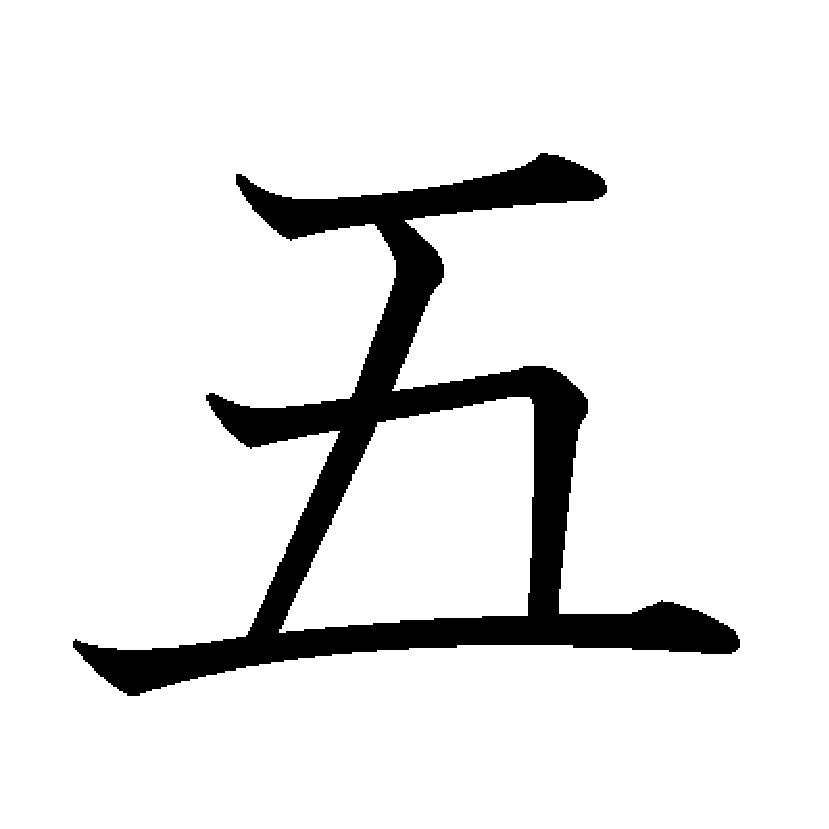
\includegraphics[width=4cm]{five.pdf}} & {
\includegraphics[width=4cm]{eye.pdf}} & {
\includegraphics[width=4cm]{woman.pdf}} \\
		{
\includegraphics[width=4cm]{large.pdf}} & {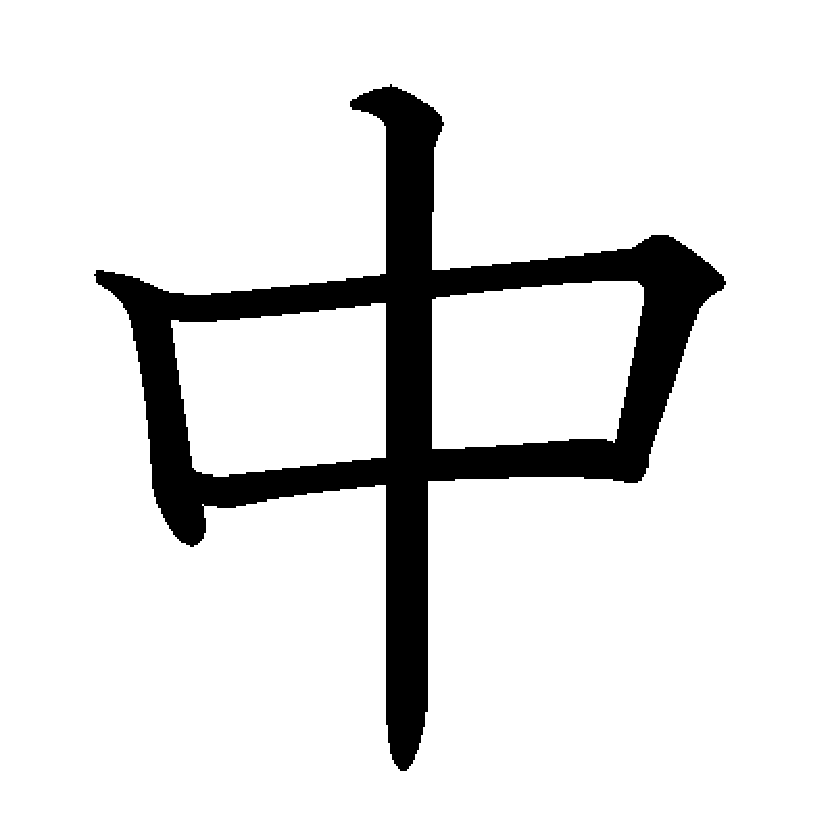
\includegraphics[width=4cm]{middle.pdf}} & {
\includegraphics[width=4cm]{eight.pdf}} & {
\includegraphics[width=4cm]{small.pdf}} \\
	};
\end{tikzpicture}
\end{document}

%
%\node (chap)
%	[
%		anchor=south west,
%		color=black,
%		outer sep=0,
%		font=\huge
%	]
%		at (m.north west)
%	{
%		\textbf{\lmr Chapter 1}
%	};